\documentclass[10pt,twocolumn]{article}

\usepackage[letterpaper,margin=0.68in,columnsep=0.24in]{geometry}
\usepackage[T1]{fontenc}
\usepackage[utf8]{inputenc}
\usepackage{lmodern}
\usepackage{microtype}
\usepackage{amsmath,amssymb}
\usepackage{booktabs}
\usepackage{tabularx}
\usepackage{array}
\usepackage{enumitem}
\usepackage{xcolor}
\usepackage{tikz}
\usepackage{hyperref}

\definecolor{trviolet}{HTML}{7257D8}
\definecolor{trblue}{HTML}{277DA1}
\definecolor{trgreen}{HTML}{2A9D8F}
\definecolor{tramber}{HTML}{D98E04}
\definecolor{trgray}{HTML}{4E5968}

\hypersetup{
  colorlinks=true,
  linkcolor=trviolet,
  citecolor=trblue,
  urlcolor=trblue,
  pdftitle={TR-Hash 200M: Multi-Hash Routing Across 162B Token Exposures and Full-Parameter SFT},
  pdfauthor={Boris Peyriguere},
  pdfsubject={Released architecture, training lineage, PIQA evaluation, and limitations},
  pdfkeywords={mixture of experts, deterministic routing, token identity, supervised fine-tuning, PIQA}
}

\setlist{nosep,leftmargin=*}
\setlength{\parindent}{1em}
\setlength{\parskip}{0pt}

\newcommand{\model}{TR-Hash 200M}
\newcommand{\code}[1]{\texttt{#1}}
\newcommand{\metric}[1]{\textbf{#1}}

\title{\vspace{-1.2em}\textbf{TR-Hash 200M: Multi-Hash Token Routing Across\\162B Token Exposures and Full-Parameter SFT}}
\author{Boris Peyriguere\\\small Complexity-ML, Independent Research\\\small \href{mailto:boris@complexity-ai.fr}{boris@complexity-ai.fr}}
\date{August 2026}

\begin{document}
\maketitle

\begin{abstract}
We report the released training lineage of \model, a 201.2M-parameter decoder-only language model whose feed-forward blocks combine an always-on shared SwiGLU path with four deterministic token-ID-routed residual experts, two active per token. Routing is compiled once per layer by multi-hash rendezvous voting; it has no learned gate and adds no runtime routing model. The lineage comprises (i) a completed 129.996B-token replay-scheduled base pretraining run, (ii) a fresh-optimizer full-parameter refinement stopped at step 8,156 after 32.069B additional unique-token exposures, and (iii) three epochs of full-parameter supervised fine-tuning (SFT) on an audited 300,000-example v2 mixture with 202.949M tokenized training tokens per epoch. On the full 1,838-example PIQA validation split, zero-shot causal continuation scoring without a chat template moves from 65.45/65.61 accuracy/length-normalized accuracy for the base checkpoint to 68.66/68.39 after refinement and 68.01/69.10 for the released SFT epoch-3 checkpoint. Matched held-out SFT loss decreases from 1.7226 before SFT to 0.9596 after epoch 3. These are single-lineage results without a parameter-matched dense or learned-router control, multi-seed replication, or contamination audit; they establish a reproducible released artifact, not architectural superiority.
\end{abstract}

\section{Introduction}
Learned mixture-of-experts (MoE) routers condition parameter selection on the current hidden state, but quality, capacity, dispatch, router optimization, and balancing objectives then change together~\cite{shazeer2017outrageously,fedus2022switch,jiang2024mixtral}. Fixed token-ID routing is a deliberately narrower intervention: attention continues to build contextual hidden states, while lexical identity selects a small residual feed-forward subspace. The selection can be persisted, audited, and reproduced independently of activations or training progress.

This paper updates the earlier architecture-and-plan report for \model. That report intentionally contained no training result because the base run was unfinished. The present version records the realized three-stage lineage, the released checkpoint selected after full-parameter SFT, and the limits of the evidence. It does not fold the earlier experimental LoRA work into the release: all weights in the promoted assistant were updated by full-parameter SFT.

The contributions are:
\begin{enumerate}
  \item an exact description of the released 201.2M multi-hash shared-plus-residual architecture;
  \item an auditable accounting of 129.996B base exposures, 32.069B refinement exposures, and 608.846M tokenized SFT exposures across three epochs;
  \item checkpoint-level PIQA results under one fixed zero-shot continuation protocol; and
  \item explicit separation of training minibatch loss, matched SFT validation loss, downstream accuracy, and qualitative chat behavior.
\end{enumerate}

\section{Architecture}
\subsection{Contextual backbone}
The model is a pre-norm causal decoder with 16 Transformer layers, hidden size 896, RMSNorm, rotary position embeddings, query/key normalization, and tied input/output embeddings. Grouped-query attention (GQA) uses 14 query heads and two key/value heads~\cite{ainslie2023gqa,su2021roformer}. The vocabulary has 32,000 entries and the configured maximum sequence length is 2,048 tokens.

\begin{table}[t]
\centering
\caption{Released architecture. Stored parameters include all four routed experts; two are active for each token.}
\label{tab:architecture}
\small
\begin{tabular}{@{}lr@{}}
\toprule
Component & Value \\
\midrule
Trainable parameters & 201,194,368 \\
Layers / hidden size & 16 / 896 \\
GQA query / KV heads & 14 / 2 \\
Vocabulary / context & 32,000 / 2,048 \\
Shared SwiGLU width & 3,072 \\
Stored experts / width & 4 / 64 \\
Active experts & top-2 \\
Routing channels & 2 hashes \\
\bottomrule
\end{tabular}
\end{table}

\subsection{Shared and routed computation}
Let $x_l$ be a contextual hidden state at layer $l$, $t$ its token ID, $S_l$ the shared SwiGLU branch, and $E_{l,e}$ one of four residual experts. A persisted table $R_l \in \{0,1,2,3\}^{2\times 32{,}000}$ supplies two distinct experts. The realized feed-forward output is
\begin{equation}
F_l(x_l,t)=S_l(x_l)+2\sum_{j=1}^{2}0.5\,E_{l,R_{l,j}(t)}(x_l).
\end{equation}
Thus the routed contribution is the sum of the two selected expert outputs. The shared branch remains active for every token and is substantially wider than each expert. In the public configuration, \texttt{intermediate\_size=256} denotes total routed width: four width-64 experts are stored, and top-2 activates 128 routed channels. Stored intermediate width is therefore $3072+4\times64=3328$; active intermediate width is $3072+2\times64=3200$. Expert tensors account for 5.47\% of model parameters.

\subsection{Multi-hash route construction}
For every layer, token/expert pairs receive two independent 32-bit rendezvous scores. Scores are summed across hash channels, and the two experts with the largest totals become the token's fixed routes. The result is compiled into the ordinary $[\mathrm{top\mbox{-}k},\mathrm{vocab}]$ dispatch table. Consequently, multi-hash construction adds no per-token learned routing network and no additional scoring operation during inference.

The exported tables are training-independent. Across the 16 layers, route tables are pairwise distinct and no token selects the same expert twice. In the first layer, expert occupancy is 15,954 / 16,118 / 15,917 / 16,011 of 64,000 total route slots, each within 0.7\% of the uniform target. This is marginal balance over the vocabulary, not a claim that ordered expert pairs or runtime corpus traffic are uniform. Fixed lexical hashes as routing signals relate to Hash Layers~\cite{roller2021hash}; the always-on shared path is also consistent with the motivation behind shared-expert MoE designs~\cite{dai2024deepseekmoe}.

\section{Training Lineage}
\begin{figure*}[t]
\centering
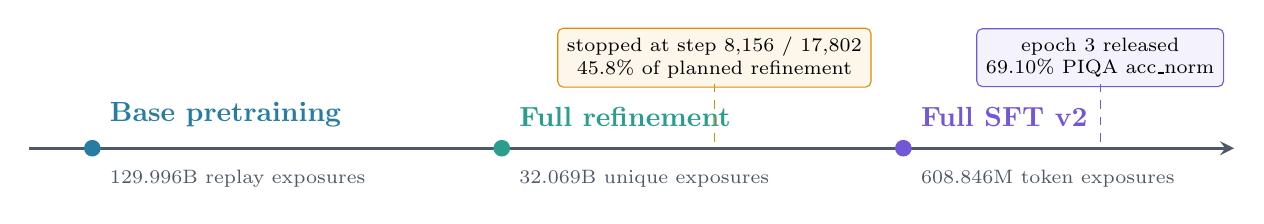
\begin{tikzpicture}[font=\small,>=stealth]
  \draw[->,line width=1.2pt,trgray] (0,0) -- (15.3,0);
  \foreach \x/\c/\title/\sub in {
    0.8/trblue/{Base pretraining}/{129.996B replay exposures},
    6.0/trgreen/{Full refinement}/{32.069B unique exposures},
    11.1/trviolet/{Full SFT v2}/{608.846M token exposures}}
  {
    \fill[\c] (\x,0) circle (3pt);
    \node[anchor=south west,text=\c,font=\bfseries] at (\x+0.1,0.15) {\title};
    \node[anchor=north west,text=trgray,font=\scriptsize] at (\x+0.1,-0.15) {\sub};
  }
  \node[draw=tramber,rounded corners=2pt,fill=tramber!8,align=center,font=\scriptsize] at (8.7,1.15) {stopped at step 8,156 / 17,802\\45.8\% of planned refinement};
  \draw[tramber,dashed] (8.7,0.82) -- (8.7,0.05);
  \node[draw=trviolet,rounded corners=2pt,fill=trviolet!8,align=center,font=\scriptsize] at (13.6,1.15) {epoch 3 released\\69.10\% PIQA acc\_norm};
  \draw[trviolet,dashed] (13.6,0.82) -- (13.6,0.05);
\end{tikzpicture}
\caption{Released lineage. The ``160B'' repository name is a rounded label for approximately 162.065B source-token exposures; it does not imply that the planned 70B-token refinement completed.}
\label{fig:lineage}
\end{figure*}

\subsection{Stage 1: replay-scheduled base pretraining}
The base run selects 70B unique tokens from a larger immutable, pretokenized mixture and uses source-specific replay counts to target 130B exposures. Sources include DCLM, FineWeb-Edu-Dedup, Stack-Edu, FineMath, InfiWebMath, and Cosmopedia v2. The run completes 165,298 optimizer steps and 129,995,636,736 token exposures. Its last logged training minibatch has loss 2.652628 and token-level perplexity 14.19 at learning rate $3\times10^{-5}$. Because this is a final minibatch rather than a held-out corpus estimate, it is reported as an execution record, not as a generalization metric.

\subsection{Stage 2: full-parameter refinement}
Refinement starts from base weights only, with a fresh optimizer and learning-rate schedule. It revisits the same 70B unique-token selection without replay or augmentation. The run is stopped at step 8,156 of 17,802 after approximately 32,069,495,945 additional source-token exposures (45.8\% of the planned pass). The terminal progress display records training loss 2.3208 and perplexity 10.2. The release therefore preserves an evaluated intermediate checkpoint; no process is expected to complete the remaining refinement steps.

\subsection{Stage 3: full-parameter instruction SFT}
Instruction post-training starts from the step-8,156 refinement checkpoint. The model is trained for three epochs over the audited SFT v2 mixture: 300,000 training examples and 3,000 held-out examples, encoded with the released 32,000-token tokenizer and capped at the native 2,048-token context without truncation. The training split contains 202,948,693 tokenized tokens per epoch. It covers general instruction following, verified mathematics, execution-filtered code, constraints, rewriting, summarization, STEM, short multi-turn conversation, and English/French bilingual instruction. The \code{complexity-chat-v2} template is used for SFT and chat serving. All model parameters are optimized; this stage is not LoRA or QLoRA.

The held-out SFT set contains 981,892 supervised tokens and is evaluated at the source checkpoint and each epoch boundary. Table~\ref{tab:sftloss} shows monotonic improvement through epoch 3. Epoch 3 also records the strongest normalized PIQA result of the three candidates and is copied to the root F32 SafeTensors release.

\begin{table}[t]
\centering
\caption{Matched held-out SFT evaluation. Perplexity is $\exp(\mathrm{loss})$.}
\label{tab:sftloss}
\small
\begin{tabular}{@{}lrrr@{}}
\toprule
Checkpoint & Step & Loss & PPL \\
\midrule
SFT source & 0 & 1.722610 & 5.60 \\
Epoch 1 & 1,994 & 0.990943 & 2.69 \\
Epoch 2 & 3,988 & 0.963912 & 2.62 \\
Epoch 3 & 5,982 & \textbf{0.959617} & \textbf{2.61} \\
\bottomrule
\end{tabular}
\end{table}

\section{\hspace{0.3em}Evaluation}
\subsection{PIQA protocol}
We evaluate the full 1,838-example PIQA validation split~\cite{bisk2020piqa}. Each candidate ending is scored as a causal continuation of the prompt. Accuracy selects the higher total log-likelihood; normalized accuracy selects the higher length-normalized log-likelihood. The protocol is zero-shot, uses no chat template, and caps sequences at 2,048 tokens. The same checkpoint weights are evaluated in FP16 through MLX. This continuation protocol avoids confounding the result with chat-template behavior.

\begin{table*}[t]
\centering
\caption{PIQA validation results for the released lineage. ``Source exposure'' excludes the 608.846M tokenized SFT exposures. No significance test or multi-seed interval is claimed.}
\label{tab:piqa}
\small
\begin{tabularx}{\textwidth}{@{}l>{\raggedleft\arraybackslash}p{1.35in}>{\raggedleft\arraybackslash}p{0.72in}>{\raggedleft\arraybackslash}p{0.85in}X@{}}
\toprule
Checkpoint & Source-token exposure & PIQA acc & PIQA acc\_norm & Release interpretation \\
\midrule
Base final, step 165,298 & 129.996B & 65.45\% & 65.61\% & Completed replay-scheduled base model \\
Refinement, step 8,156 & 162.065B & 68.66\% & 68.39\% & Interrupted full-parameter intermediate \\
Full SFT v2, epoch 3 & 162.065B + SFT & \textbf{68.01\%} & \textbf{69.10\%} & Released root assistant checkpoint \\
\bottomrule
\end{tabularx}
\end{table*}

Refinement provides the largest observed PIQA change relative to the released base: +3.21 points in accuracy and +2.78 points in normalized accuracy. Full SFT v2 retains that improvement and changes PIQA by -0.65 / +0.71 points relative to refinement. PIQA does not measure instruction following, safety, code generation, or open-ended chat quality; it is used here as a narrow checkpoint-selection sanity check.

\subsection{What the losses mean}
The three loss signals in this report have different sampling processes. The base and refinement numbers are terminal training displays from autoregressive corpus training. Table~\ref{tab:sftloss} is a matched held-out SFT evaluation over supervised labels. Table~\ref{tab:piqa} is a discrete multiple-choice continuation benchmark. A lower SFT loss does not guarantee a higher PIQA score, and none of these numbers alone establishes assistant quality.

\section{Implementation and Release Artifacts}
The canonical implementation is maintained in the open-source Complexity Framework. The TR-Hash engine exposes a universal PyTorch path, optional Triton/CUDA grouped dispatch, and a CUDA-graph inference path while preserving the same persisted routes. The release includes configuration, tokenizer assets, Safetensors weights, model cards, training logs where available, and an OpenAI-compatible serving stack in TR-Hash-i64.

The released epoch-3 checkpoint is exported as F32 SafeTensors at the model repository root; its exact SHA-256 is recorded in the accompanying release manifest. The release is available at \url{https://huggingface.co/AETHORIA-AI/TR-HASH-MoE-200M-160B-SFT}; the base and refinement repositories retain their distinct roles. The public chat at \url{https://www.complexity-ai.fr/ai-lab} loads the released full-SFT model. Experimental LoRA repositories are not part of this lineage.

An interactive 3-D t-SNE artifact probes routed residual contributions on natural PIQA text. It samples two routed contribution vectors per token from layers 1, 4, 8, 12, and 16, excludes the shared branch, L2-normalizes vectors, and applies PCA followed by t-SNE. This is an exploratory inspection tool, not evidence of semantic specialization or quality.

\section{Limitations and Responsible Use}
This study has one architecture, one training lineage, and no parameter-matched dense or learned-router control. It does not isolate whether the PIQA change comes from additional token exposure, data order, schedule, or the routing architecture. There is no multi-seed replication, statistical significance test, benchmark-contamination audit, memorization analysis, toxicity study, bias audit, or systematic safety evaluation.

The model is small and experimental. It may hallucinate, repeat, refuse benign requests, comply with unsafe requests, emit biased content, fail arithmetic or code, and lose coherence over long contexts. The public chat is a research demonstration, not a reliable agent or decision system. The CC BY-NC 4.0 model license does not replace source-dataset terms; users remain responsible for provenance and compliance.

\section{Conclusion}
\model{} demonstrates that a 201.2M-parameter decoder with fixed, multi-hash token-ID routing can be trained end to end through a long base run, continued with fresh-optimizer full-parameter refinement, and converted into an instruction-tuned assistant by full-parameter SFT. The released SFT v2 epoch-3 checkpoint improves PIQA acc\_norm from 65.61\% at the base endpoint to 69.10\% and reaches a matched held-out SFT loss of 0.959617. The result is best read as a transparent artifact lineage with precise accounting and known limits, not as proof that deterministic routing outperforms dense or learned alternatives.

\paragraph{Reproducibility.}
Code: \url{https://github.com/Complexity-ML/complexity-framework}. Runtime: \url{https://github.com/Complexity-ML/TR-Hash-i64}. Model collection: \url{https://huggingface.co/AETHORIA-AI}.

\paragraph{Use of generative AI tools.}
Generative AI tools assisted with language editing, consistency checks against author-provided configuration and measured artifacts, and PDF packaging. The author reviewed the numerical claims and takes responsibility for the final text.

\begin{thebibliography}{9}
\bibitem{ainslie2023gqa}
J. Ainslie et al. GQA: Training Generalized Multi-Query Transformer Models from Multi-Head Checkpoints. \emph{arXiv:2305.13245}, 2023.

\bibitem{bisk2020piqa}
Y. Bisk et al. PIQA: Reasoning about Physical Commonsense in Natural Language. \emph{AAAI}, 2020.

\bibitem{dai2024deepseekmoe}
D. Dai et al. DeepSeekMoE: Towards Ultimate Expert Specialization in Mixture-of-Experts Language Models. \emph{ACL}, 2024.

\bibitem{fedus2022switch}
W. Fedus, B. Zoph, and N. Shazeer. Switch Transformers: Scaling to Trillion Parameter Models with Simple and Efficient Sparsity. \emph{JMLR}, 23(120), 2022.

\newpage

\bibitem{jiang2024mixtral}
A. Q. Jiang et al. Mixtral of Experts. \emph{arXiv:2401.04088}, 2024.

\bibitem{roller2021hash}
S. Roller, S. Sukhbaatar, A. Szlam, and J. Weston. Hash Layers for Large Sparse Models. \emph{NeurIPS}, 2021.

\bibitem{shazeer2017outrageously}
N. Shazeer et al. Outrageously Large Neural Networks: The Sparsely-Gated Mixture-of-Experts Layer. \emph{ICLR}, 2017.

\bibitem{su2021roformer}
J. Su et al. RoFormer: Enhanced Transformer with Rotary Position Embedding. \emph{arXiv:2104.09864}, 2021.
\end{thebibliography}

\end{document}
